\documentclass[11pt,fleqn]{article}
\usepackage{graphicx}
\usepackage[letterpaper, margin=1in]{geometry}
\usepackage{hyperref}
\usepackage{multicol}
\usepackage[toc,page]{appendix}
\usepackage{amsmath}

\hypersetup{colorlinks=true, linktoc=all, linkcolor=blue}

\begin{document}

\begin{center}
\Large{\textbf{Stereo Vision Report}}\\[5pt]
\large{Robert Washbourne}\\
Last edited: \today
\end{center}

\tableofcontents

\section{Introduction}

Imagine driving in the dark, alert but not noticing a deer cross the road. Using stereo matching methods to see what is close, your car could detect the deer and brake before you even saw the obstacle. The cameras would find distances, and sensing something closer than 20 feet, send the location of the deer to the computer. The computer would see that driving over this would be catastrophic for the car, and turn on the brakes. The deer, and you, would be safe.

\section{What is Stereo Matching}

Stereo matching is a topic in computer vision where two images, taken from aligned cameras several centimetres apart, are processed and depth data is returned. For example, taking two images and using a simple algorithm, a grayscale image is returned, with lighter pixels closer then darker pixels.[6pt]  See figure \ref{fig:example1} for an example.\\

%\begin{tabular}{ccc}\\
%\hline
%\texttt{Left} & \texttt{Right} & \texttt{Disparity} \\
%\end{tabular}

%\newpage
%\begin{figure}[!ht]
%\centering
%a) 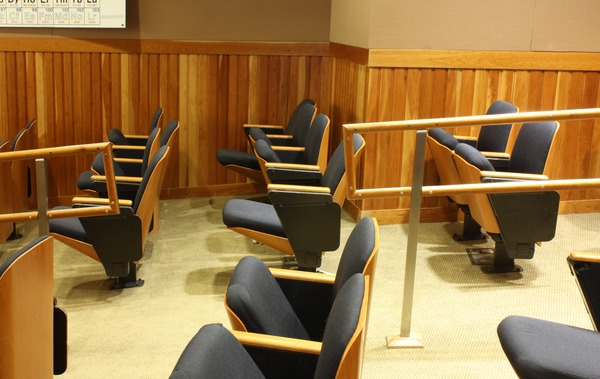
\includegraphics[width=0.6\textwidth]{images/im0-600.jpg} \\[10pt]
%b) 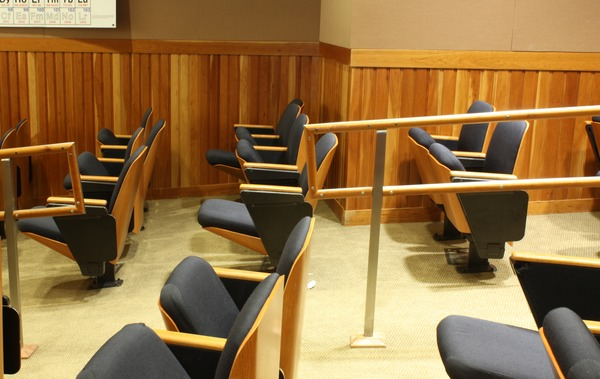
\includegraphics[width=0.6\textwidth]{images/im1-600.jpg} \\[10pt]
%c) 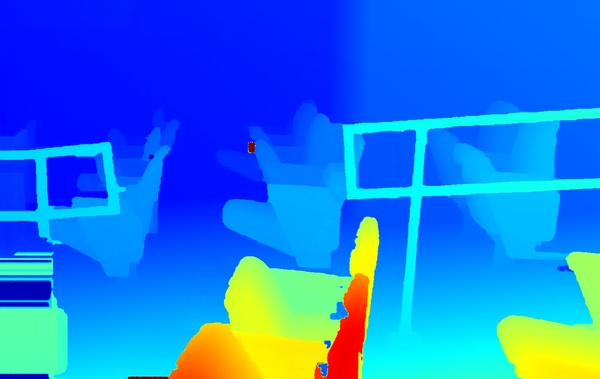
\includegraphics[width=0.6\textwidth]{images/disp-600.jpg} \\[10pt]
%\label{fig:example1}
%\caption{Example of disparity matching. a) image from left camera b) image from right camera c) disparity map}
%\end{figure}

\begin{figure}[!ht]
\centering
\setlength\tabcolsep{0.005\textwidth}
\begin{tabular}{ccc}
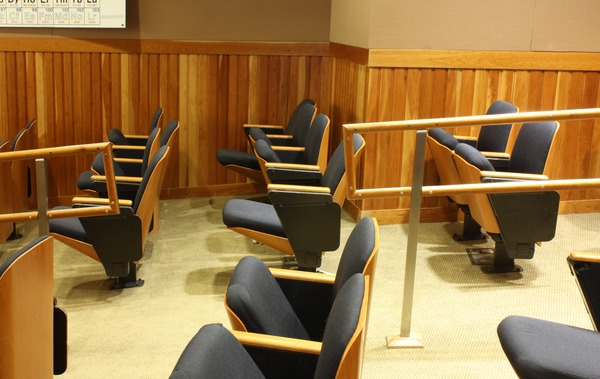
\includegraphics[width=0.33\textwidth]{images/im0-600.jpg} &
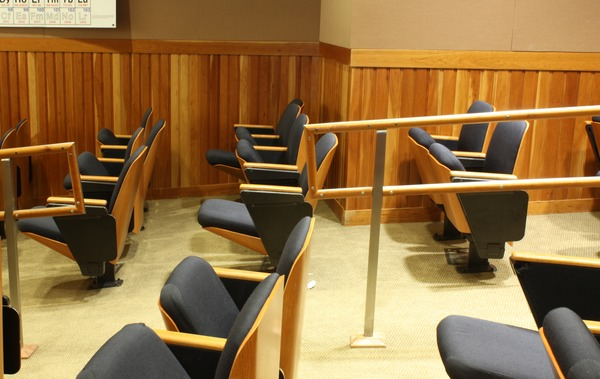
\includegraphics[width=0.33\textwidth]{images/im1-600.jpg} &
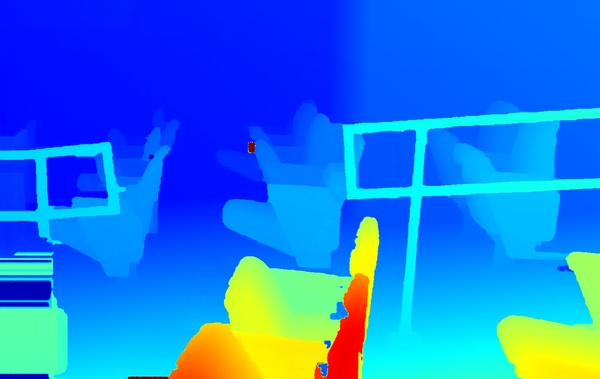
\includegraphics[width=0.33\textwidth]{images/disp-600.jpg} \\[2pt]
a) & b) & c) \\
\end{tabular}
\caption{Example of disparity matching. a) Image from left camera. b) Image from right camera c) Disparity map.}
\label{fig:example1}
\end{figure}




\section{Methods}
There are several methods of creating depth maps.
They can be created by a laser scanner, but this process is much slower than stereo matching, and unsuited for real time processing. They can also be created with two cameras. This is the method that I explored, as it is fast enough for realtime processing, and yields good results. In this image, a colormap is used to make it easier to see what is closer. The blues are at the back and the reds at at the front.

\subsection{Result Comparison}
\begin{figure}[!ht]
\centering
\setlength\tabcolsep{0.005\textwidth}
\begin{tabular}{ccc}
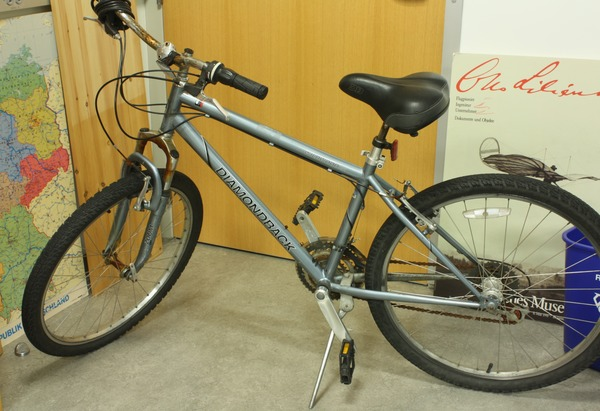
\includegraphics[width=0.33\textwidth]{images/_im0-600.jpg} &
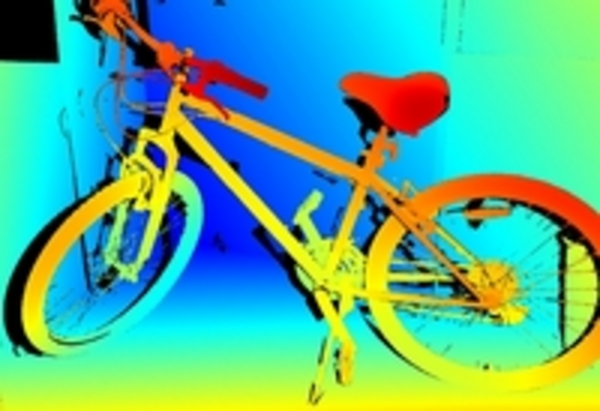
\includegraphics[width=0.33\textwidth]{images/disp0GT-600.jpg} &
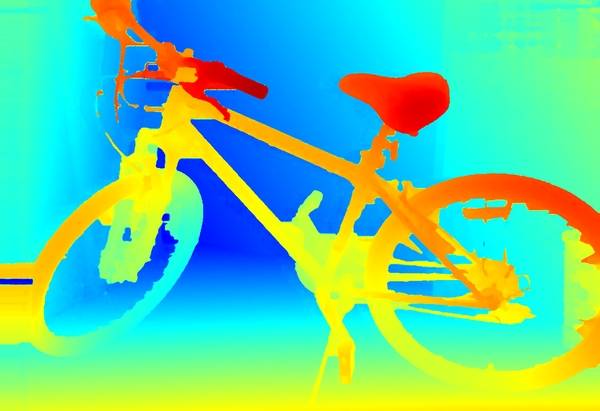
\includegraphics[width=0.33\textwidth]{images/_disp-600.jpg} \\[2pt]
a) & b) & c) \\
\end{tabular}
\caption{Comparison of laser and stereo. a) Original image b) Laser result c) Stereo matching result.}
\label{fig:result1}
\end{figure}
\\
The laser result is crisper, but it takes much longer to generate. The stereo matching result is worse, with parts of the image blended, but it was generated much faster. 

%I'd still (Dedra) like to see you do a rough time comparison here - i.e. minutes for laser and seconds for stereo...

\section{Workflow}

\subsection{Capture images from both webcams}  

%say something about this - even if it's just 'use an import command...'

\subsection{Split images into 1 pixel high rows}

The figure below (Fig. 3) is a comparison of a single row from the left image and a single row of the right image. 

%state what the y and the x axis are, and tie into next line, i.e., the x-axis is the pixel count , and since the curves are shifted ...

The data is shifted by around 60 pixels everywhere on the line.
\\

\begin{figure}[!ht]
\label{fig:strips}
\centering
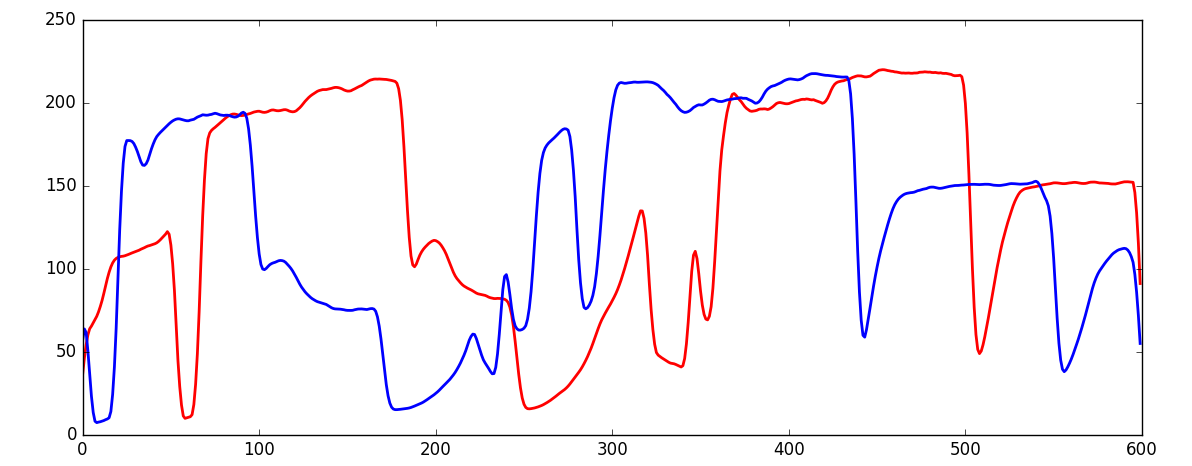
\includegraphics[width=1\textwidth]{images/strips.png} \\[2pt]
\caption{1 pixel strips from the images shown in Figure \ref{fig:example1}. Left image blue line, and right image red line. Left axis is the pixels value of the point of the bottom axis. For example, at 300, the blue line is around 200.}
\end{figure}

\subsection{Correlate image strips from left and right images}
For each pixel in the row of the left image, a window is slid along the right image's row to find a match for that pixel.\\
\\
If we did it for the 100th pixel of the blue line in the rows in figure 2, we would find that the corresponding red point is 80 pixels to the right.

\subsection{Estimate pixel distance}
The pixel distance found in the previous step is then added to the relevant row of the disparity matrix.

\subsection{Apply edge preserving filter to remove noise}
Using a median filter, a lot of noise can be removed. A median filter is a square window that centers around every pixel, and changes each pixel to the median of all the pixels inside the square.\\
For example, consider a 3 by 3 pixel median filter, which passes over a part of the image given by the values in the 4 x 4 matrix shown below. The pixel in position 2,2 has a value of 4 and is surrounded by the matrix (2, 0, 3; 1, 4, 2; 3, 1, 0).  The average value of these 9 pixels is 16/9 which rounds to 2, so the value of this pixel (originally 4) is replaced by 2.  This is a standard 'smoothing' technique.  \\
\\
A more complete example is given below:
\[ \left( \begin{array}{cccc}
2 & 0 & 3 & 5 \\
1 & 4 & 2 & 7 \\
3 & 1 & 0 & 3 \\
6 & 8 & 4 & 2 \\ 
\end{array} \right)
\rightarrow
\left(\begin{array}{ccc}
2 & 0 & 3 \\
1 & 4 & 2 \\
3 & 1 & 0 \\
\end{array} \right)
\left(\begin{array}{ccc}
0 & 3 & 5 \\
4 & 2 & 7 \\
1 & 0 & 3 \\
\end{array} \right)
\left(\begin{array}{ccc}
4 & 2 & 7 \\
1 & 0 & 3 \\
8 & 4 & 2 \\
\end{array} \right)
\left(\begin{array}{ccc}
1 & 4 & 2 \\
3 & 1 & 0 \\
6 & 8 & 4 \\
\end{array} \right)\]
We see that the medians of the 3x3 matrixes are
\begin{equation} \label{eq1}
\begin{split}
(0,0,1,1,2,2,3,3,4) &=  2\\
(0,0,1,2,3,3,4,5,7) &=  3\\
(0,1,2,2,3,4,4,7,8) &=  3\\
(0,1,1,2,3,4,4,6,8) &=  3.\\
\end{split}
\end{equation}
So our matrix changed from $\left(\begin{array}{cc}
4 & 2 \\
1 & 0 \\
\end{array} \right)$ to $\left(\begin{array}{cc}
2 & 3 \\
3 & 3 \\
\end{array} \right)$.

On a larger scale, results are a lot more interesting. Here are some results from my code:\\

\begin{tabular}{ccc}
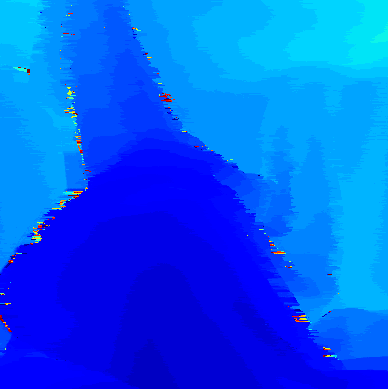
\includegraphics[width=0.456\textwidth]{images/withoutmedianfilter.png} &
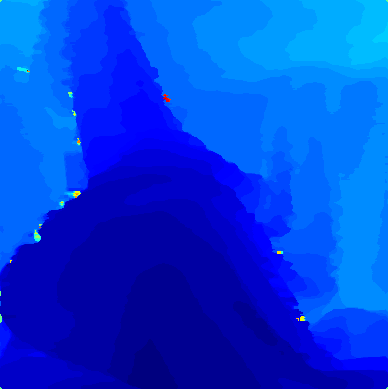
\includegraphics[width=0.456\textwidth]{images/withmedianfilter.png}\\[2pt]
Without median filter & With median filter \\
\end{tabular}

\subsection{Return the final disparity map}

The disparity map matrix values do not show actual distance. To turn these values into distances, my program uses a triangulation method based on knowing the distance between cameras.
\begin{center}
\begin{tabular}{cc}
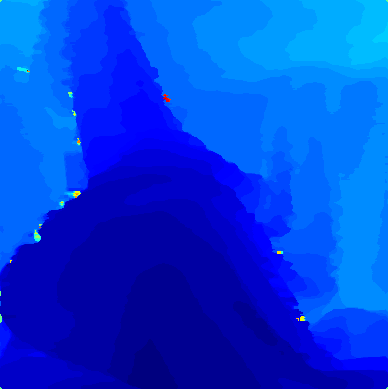
\includegraphics[width=0.6\textwidth]{images/withmedianfilter.png}\\
Final result
\end{tabular}
\end{center}

\section{Setup}
My setup is a wooden board with 2 Microsoft LifeCam 3000 webcams 2 centimeters apart, facing the same direction. It can resolve the depths of objects that are farther than three feet away, and works both indoors and outdoors.\\[2pt]

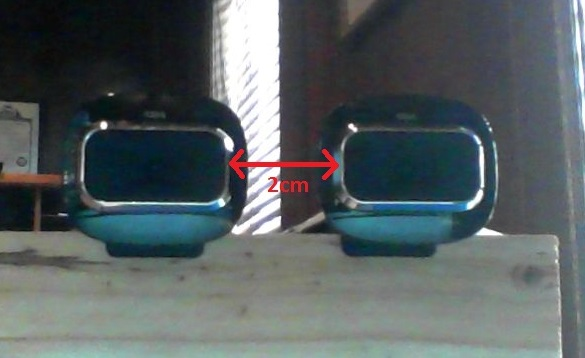
\includegraphics[width=0.8\textwidth]{images/setup.jpg}


\begin{appendices}

% ........................................................................................................................
\section{References}
% ........................................................................................................................

\begin{enumerate}
\item Middlebury Computer Vision dataset for the example images and laser vs stereo matching comparison. (http://vision.middlebury.edu)
\item Image used in figure \ref{fig:example1}\\ http://vision.middlebury.edu/stereo/datasets3/test/Classroom2/im0-600.jpg
\item Image used in figure \ref{fig:example1}\\ http://vision.middlebury.edu/stereo/datasets3/test/Classroom2/im1-600.jpg
\item Image used in figure \ref{fig:example1}\\ http://vision.middlebury.edu/stereo/results3/outputs/alg0034/test/Classroom2/disp-600.jpg
\end{enumerate}


% ........................................................................................................................
\section{Definitions}
% ........................................................................................................................
\begin{itemize}
\item \texttt{Computer Vision}\\[2pt]
The field of acquiring, processing, analyzing, and understanding data from the real world.

\item \texttt{Stereo Matching}\\[2pt]
The method to create disparity maps. Part the field of computer vision.

\item \texttt{Disparity Maps}\\[2pt]
Grayscale images that represent distance in an image. Can be converted to a 3D point cloud without too much trouble.
\end{itemize}

\end{appendices}

\end{document}